\documentclass[preview]{standalone}
\usepackage{amsmath}
\usepackage{tikz}
\usepackage{mathdots}
\usepackage{yhmath}
\usepackage{cancel}
\usepackage{color}
\usepackage{xcolor}
\usepackage{siunitx}
\usepackage{array}
\usepackage{multirow}
\usepackage{amssymb}
\usepackage{gensymb}
\usepackage{tabularx}
\usepackage{extarrows}
\usepackage{booktabs}
\usetikzlibrary{fadings}
\usetikzlibrary{patterns}
\usetikzlibrary{shadows.blur}
\usetikzlibrary{shapes}
\begin{document}
\begin{center}




\tikzset{every picture/.style={line width=0.75pt}} %set default line width to 0.75pt        

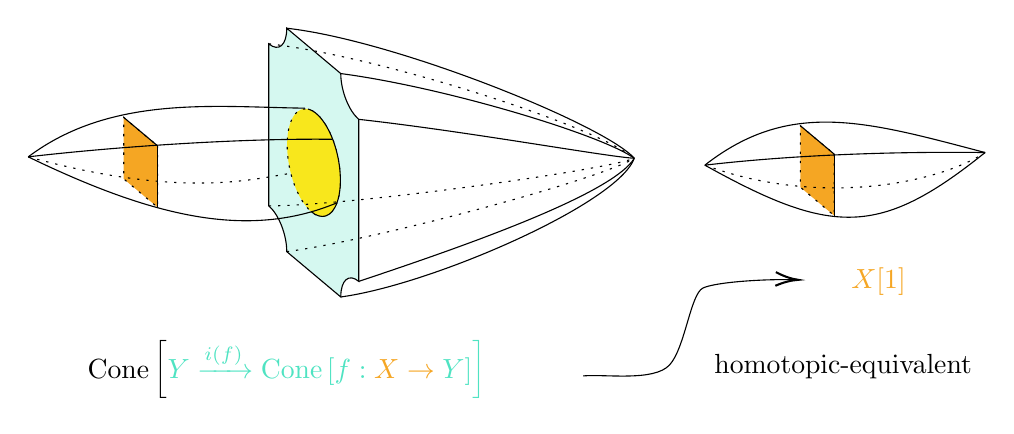
\begin{tikzpicture}[x=0.75pt,y=0.75pt,yscale=-1,xscale=1]
%uncomment if require: \path (0,205); %set diagram left start at 0, and has height of 205

%Shape: Plaque [id:dp4672044207967565] 
\draw  [fill={rgb, 255:red, 80; green, 227; blue, 194 }  ,fill opacity=0.24 ] (202.55,19) .. controls (207.35,23.02) and (211.23,19.66) .. (211.23,11.49) -- (237.25,33.33) .. controls (237.25,41.5) and (241.14,51.37) .. (245.93,55.39) -- (245.93,133.46) .. controls (241.14,129.44) and (237.25,132.8) .. (237.25,140.96) -- (211.23,119.13) .. controls (211.23,110.96) and (207.35,101.09) .. (202.55,97.07) -- cycle ;
%Shape: Arc [id:dp48772527335668436] 
\draw  [draw opacity=0][fill={rgb, 255:red, 248; green, 231; blue, 28 }  ,fill opacity=1 ][dash pattern={on 0.84pt off 2.51pt}] (235.42,95.6) .. controls (235.42,95.6) and (235.42,95.6) .. (235.42,95.6) .. controls (231.95,105.13) and (224.14,104.19) .. (217.96,93.49) .. controls (211.78,82.79) and (209.59,66.39) .. (213.06,56.86) .. controls (216.53,47.33) and (224.35,48.27) .. (230.52,58.97) .. controls (236.6,69.49) and (238.82,85.52) .. (235.59,95.11) -- (224.24,76.23) -- cycle ; \draw  [dash pattern={on 0.84pt off 2.51pt}] (235.42,95.6) .. controls (235.42,95.6) and (235.42,95.6) .. (235.42,95.6) .. controls (231.95,105.13) and (224.14,104.19) .. (217.96,93.49) .. controls (211.78,82.79) and (209.59,66.39) .. (213.06,56.86) .. controls (216.53,47.33) and (224.35,48.27) .. (230.52,58.97) .. controls (236.6,69.49) and (238.82,85.52) .. (235.59,95.11) ;  
%Shape: Rectangle [id:dp9250708704645467] 
\draw  [color={rgb, 255:red, 0; green, 0; blue, 0 }  ,draw opacity=1 ][fill={rgb, 255:red, 245; green, 166; blue, 35 }  ,fill opacity=1 ][dash pattern={on 0.84pt off 2.51pt}] (149,68.16) -- (149,97.78) -- (132.67,84.08) -- (132.67,54.46) -- cycle ;
%Curve Lines [id:da3223234128843173] 
\draw    (86.67,73.46) .. controls (126.67,43.46) and (176.67,49.46) .. (220,50) ;
%Curve Lines [id:da5514567074328707] 
\draw  [dash pattern={on 0.84pt off 2.51pt}]  (86.67,73.46) .. controls (159.67,93.46) and (193.67,84.46) .. (212.67,81.46) ;
%Shape: Arc [id:dp9307884772604522] 
\draw  [draw opacity=0][fill={rgb, 255:red, 248; green, 231; blue, 28 }  ,fill opacity=1 ] (221.44,50.44) .. controls (224.42,51.13) and (227.65,53.99) .. (230.52,58.97) .. controls (236.7,69.67) and (238.89,86.07) .. (235.42,95.6) .. controls (232.86,102.65) and (227.9,103.97) .. (223,99.84) -- (224.24,76.23) -- cycle ; \draw   (221.44,50.44) .. controls (224.42,51.13) and (227.65,53.99) .. (230.52,58.97) .. controls (236.7,69.67) and (238.89,86.07) .. (235.42,95.6) .. controls (232.86,102.65) and (227.9,103.97) .. (223,99.84) ;  
%Curve Lines [id:da08224623949039134] 
\draw    (86.67,73.46) .. controls (129.67,68.46) and (189.67,64.46) .. (233,65) ;
%Straight Lines [id:da4184137062900761] 
\draw    (132.67,54.46) -- (149,68.16) ;
%Straight Lines [id:da7708885349783519] 
\draw    (149,68.16) -- (149,97.78) ;
%Curve Lines [id:da7761395466306564] 
\draw    (86.67,73.46) .. controls (146.67,102.46) and (192.67,113.46) .. (235.42,95.6) ;
%Curve Lines [id:da7459059590036898] 
\draw    (237.25,33.33) .. controls (288.67,40.15) and (363.67,63.15) .. (378.67,74.15) ;
%Curve Lines [id:da008287826223109418] 
\draw    (245.93,55.39) .. controls (298.34,61.21) and (363.67,73.15) .. (378.67,74.15) ;
%Curve Lines [id:da18712132225685307] 
\draw    (245.93,133.46) .. controls (291.67,118.15) and (367.67,92.15) .. (378.67,74.15) ;
%Curve Lines [id:da3248143393563616] 
\draw    (237.25,140.96) .. controls (280.67,135.15) and (370.67,96.15) .. (378.67,74.15) ;
%Curve Lines [id:da5248387577755014] 
\draw    (211.23,11.49) .. controls (263.64,17.32) and (364.67,58.15) .. (378.67,74.15) ;
%Curve Lines [id:da27866882733957454] 
\draw  [dash pattern={on 0.84pt off 2.51pt}]  (202.55,19) .. controls (254.97,24.82) and (359.67,58.15) .. (378.67,74.15) ;
%Curve Lines [id:da477690359596479] 
\draw  [dash pattern={on 0.84pt off 2.51pt}]  (211.23,119.13) .. controls (255.67,113.15) and (362.67,84.15) .. (378.67,74.15) ;
%Curve Lines [id:da03231817135097059] 
\draw  [dash pattern={on 0.84pt off 2.51pt}]  (202.55,97.07) .. controls (240.67,97.15) and (363.67,80.15) .. (378.67,74.15) ;
%Shape: Rectangle [id:dp794797175040002] 
\draw  [color={rgb, 255:red, 0; green, 0; blue, 0 }  ,draw opacity=1 ][fill={rgb, 255:red, 245; green, 166; blue, 35 }  ,fill opacity=1 ][dash pattern={on 0.84pt off 2.51pt}] (475,72.16) -- (475,101.78) -- (458.67,88.08) -- (458.67,58.46) -- cycle ;
%Curve Lines [id:da4997433117698318] 
\draw    (412.67,77.46) .. controls (453.67,45.38) and (490.67,56.38) .. (547.67,71.38) ;
%Curve Lines [id:da8475279120888364] 
\draw  [dash pattern={on 0.84pt off 2.51pt}]  (412.67,77.46) .. controls (469.67,98.38) and (526.67,85.38) .. (547.67,71.38) ;
%Curve Lines [id:da49314824814473845] 
\draw    (412.67,77.46) .. controls (455.67,72.46) and (504.33,70.83) .. (547.67,71.38) ;
%Straight Lines [id:da43225120040283693] 
\draw    (458.67,58.46) -- (475,72.16) ;
%Straight Lines [id:da06455159190324777] 
\draw    (475,72.16) -- (475,101.78) ;
%Curve Lines [id:da9104231108198488] 
\draw    (412.67,77.46) .. controls (473.67,111.38) and (496.67,112.38) .. (547.67,71.38) ;
%Curve Lines [id:da7436905598656782] 
\draw    (354,179) .. controls (364.82,178.07) and (388.24,181.81) .. (395.67,173.71) .. controls (403.09,165.61) and (405.73,139.68) .. (411.67,136.71) .. controls (417.37,133.86) and (440.66,132.26) .. (455.82,132.65) ;
\draw [shift={(457.67,132.71)}, rotate = 182.2] [color={rgb, 255:red, 0; green, 0; blue, 0 }  ][line width=0.75]    (10.93,-3.29) .. controls (6.95,-1.4) and (3.31,-0.3) .. (0,0) .. controls (3.31,0.3) and (6.95,1.4) .. (10.93,3.29)   ;

% Text Node
\draw (114,160.4) node [anchor=north west][inner sep=0.75pt]    {$\mathrm{Cone}\left[\color[rgb]{0.31,0.89,0.76}{Y}\xrightarrow{i( f)}\mathrm{Cone}\left[ f:\color[rgb]{0.96,0.65,0.14}{X}\rightarrow \color[rgb]{0.31,0.89,0.76}{Y}\right]\right]$};
% Text Node
\draw (416,167.4) node [anchor=north west][inner sep=0.75pt]    {$\text{homotopic-equivalent}$};
% Text Node
\draw (482,125.72) node [anchor=north west][inner sep=0.75pt]    {$\color[rgb]{0.96,0.65,0.14}{X}[ 1]$};


\end{tikzpicture}


\end{center}
\end{document}
